% Two-tier architecture. Build: see figures/build.sh
\documentclass[border=10pt]{standalone}
\usepackage[T1]{fontenc}
\usepackage{helvet}
\renewcommand{\familydefault}{\sfdefault}
\usepackage{tikz}
\usetikzlibrary{positioning,fit,arrows.meta,backgrounds,calc}

\definecolor{shared}{HTML}{3B6EA8}
\definecolor{light}{HTML}{1F8A70}
\definecolor{pro}{HTML}{7A4FB5}
\definecolor{ink}{HTML}{222222}
\definecolor{muted}{HTML}{666666}

\tikzset{
  box/.style={draw=#1, line width=0.9pt, rounded corners=3pt, fill=#1!7,
              align=center, inner sep=6pt, text=ink, font=\small},
  box/.default=shared,
  lane/.style={draw=#1!60, dashed, rounded corners=6pt, inner sep=9pt},
  lanelabel/.style={font=\bfseries\small, text=#1},
  arr/.style={-{Stealth[length=6pt]}, line width=0.9pt, draw=ink!70},
  note/.style={font=\scriptsize, text=muted, align=center},
}

\begin{document}
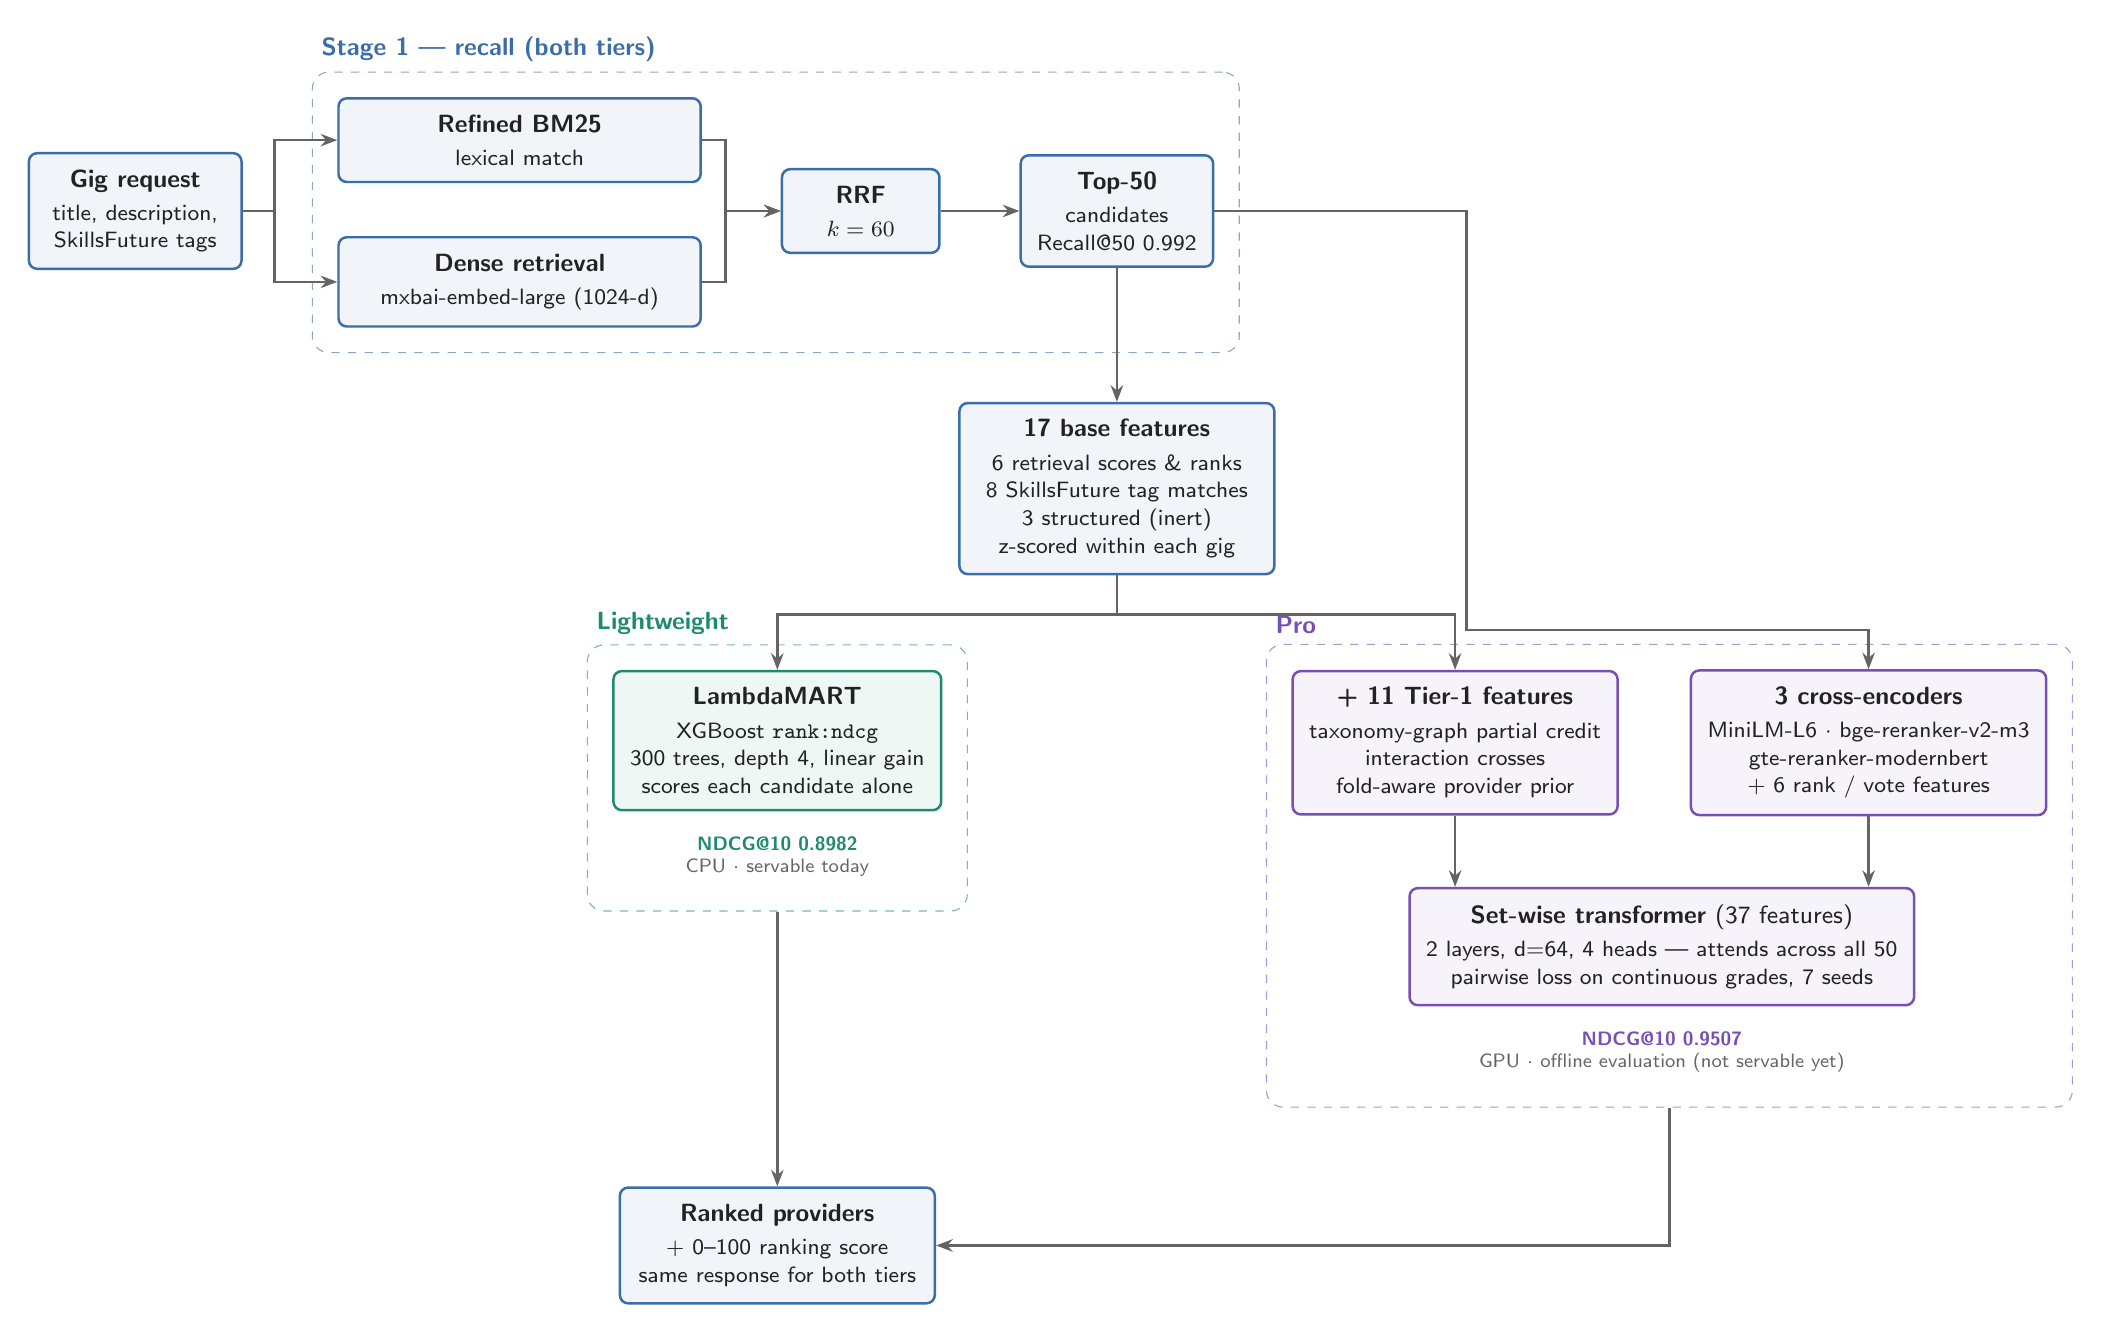
\begin{tikzpicture}[node distance=7mm and 9mm]

% ---------------- Stage 1 (shared) ----------------
\node[box, minimum width=27mm] (gig) {\textbf{Gig request}\\[1pt]\footnotesize title, description,\\[-1pt]\footnotesize SkillsFuture tags};

\node[box, right=12mm of gig, yshift=9mm, minimum width=46mm] (bm25) {\textbf{Refined BM25}\\[1pt]\footnotesize lexical match};
\node[box, right=12mm of gig, yshift=-9mm, minimum width=46mm] (dense) {\textbf{Dense retrieval}\\[1pt]\footnotesize mxbai-embed-large (1024-d)};
\node[box, anchor=west, minimum width=20mm] (rrf) at ($(bm25.east)!0.5!(dense.east)+(10mm,0)$) {\textbf{RRF}\\[1pt]\footnotesize $k=60$};
\node[box, right=10mm of rrf, minimum width=24mm] (pool) {\textbf{Top-50}\\[1pt]\footnotesize candidates\\[-1pt]\footnotesize Recall@50 0.992};

\begin{scope}[on background layer]
  \node[lane=shared, fit=(bm25)(dense)(rrf)(pool)] (s1) {};
\end{scope}
\node[lanelabel=shared, anchor=south west] at (s1.north west) {Stage 1 --- recall (both tiers)};

\draw[arr] (gig.east) -- ++(4mm,0) |- (bm25.west);
\draw[arr] (gig.east) -- ++(4mm,0) |- (dense.west);
\draw[arr] (bm25.east) -- ++(3mm,0) |- (rrf.west);
\draw[arr] (dense.east) -- ++(3mm,0) |- (rrf.west);
\draw[arr] (rrf) -- (pool);

% ---------------- base features (shared) ----------------
\node[box, below=17mm of pool, minimum width=40mm] (feat) {\textbf{17 base features}\\[1pt]
  \footnotesize 6 retrieval scores \& ranks\\[-1pt]
  \footnotesize 8 SkillsFuture tag matches\\[-1pt]
  \footnotesize 3 structured (inert)\\[-1pt]
  \footnotesize z-scored within each gig};
\draw[arr] (pool) -- (feat);

% ---------------- Lightweight lane ----------------
\node[box=light, below left=12mm and 2mm of feat, minimum width=40mm, anchor=north east] (lmart) {\textbf{LambdaMART}\\[1pt]
  \footnotesize XGBoost \texttt{rank:ndcg}\\[-1pt]
  \footnotesize 300 trees, depth 4, linear gain\\[-1pt]
  \footnotesize scores each candidate alone};
\node[note, below=2mm of lmart] (lnote) {\textbf{\color{light}NDCG@10 0.8982}\\ CPU $\cdot$ servable today};
\begin{scope}[on background layer]
  \node[lane=light, fit=(lmart)(lnote)] (llane) {};
\end{scope}
\node[lanelabel=light, anchor=south west] at (llane.north west) {Lightweight};

% ---------------- Pro lane ----------------
\node[box=pro, below right=12mm and 2mm of feat, minimum width=40mm, anchor=north west] (tier1) {\textbf{+ 11 Tier-1 features}\\[1pt]
  \footnotesize taxonomy-graph partial credit\\[-1pt]
  \footnotesize interaction crosses\\[-1pt]
  \footnotesize fold-aware provider prior};
\node[box=pro, right=9mm of tier1, minimum width=40mm] (ce) {\textbf{3 cross-encoders}\\[1pt]
  \footnotesize MiniLM-L6 $\cdot$ bge-reranker-v2-m3\\[-1pt]
  \footnotesize gte-reranker-modernbert\\[-1pt]
  \footnotesize + 6 rank / vote features};
\node[box=pro, anchor=north, minimum width=56mm] (setw) at ($(tier1.south)!0.5!(ce.south)+(0,-9mm)$) {\textbf{Set-wise transformer} (37 features)\\[1pt]
  \footnotesize 2 layers, d=64, 4 heads --- attends across all 50\\[-1pt]
  \footnotesize pairwise loss on continuous grades, 7 seeds};
\node[note, below=2mm of setw] (pnote) {\textbf{\color{pro}NDCG@10 0.9507}\\ GPU $\cdot$ offline evaluation (not servable yet)};
\begin{scope}[on background layer]
  \node[lane=pro, fit=(tier1)(ce)(setw)(pnote)] (plane) {};
\end{scope}
\node[lanelabel=pro, anchor=south west] at (plane.north west) {Pro};

\draw[arr] (feat.south) -- ++(0,-5mm) -| (lmart.north);
\draw[arr] (feat.south) -- ++(0,-5mm) -| (tier1.north);
\draw[arr] (pool.east) -- ++(32mm,0) |- ($(ce.north)+(0,5mm)$) -- (ce.north);
\draw[arr] (tier1.south) -- (tier1.south |- setw.north);
\draw[arr] (ce.south) -- (ce.south |- setw.north);

% ---------------- output ----------------
\node[box, anchor=north, minimum width=40mm] (out) at ($(llane.south |- plane.south)+(0,-10mm)$) {\textbf{Ranked providers}\\[1pt]\footnotesize + 0--100 ranking score\\[-1pt]\footnotesize same response for both tiers};
\draw[arr] (llane.south) -- (out.north);
\draw[arr] (plane.south) |- (out.east);

\end{tikzpicture}
\end{document}
